\documentclass{sigchi}

% Use this command to override the default ACM copyright statement (e.g. for preprints). 
% Consult the conference website for the camera-ready copyright statement.


%% EXAMPLE BEGIN -- HOW TO OVERRIDE THE DEFAULT COPYRIGHT STRIP -- (July 22, 2013 - Paul Baumann)
% \toappear{Permission to make digital or hard copies of all or part of this work for personal or classroom use is 	granted without fee provided that copies are not made or distributed for profit or commercial advantage and that copies bear this notice and the full citation on the first page. Copyrights for components of this work owned by others than ACM must be honored. Abstracting with credit is permitted. To copy otherwise, or republish, to post on servers or to redistribute to lists, requires prior specific permission and/or a fee. Request permissions from permissions@acm.org. \\
% {\emph{CHI'14}}, April 26--May 1, 2014, Toronto, Canada. \\
% Copyright \copyright~2014 ACM ISBN/14/04...\$15.00. \\
% DOI string from ACM form confirmation}
%% EXAMPLE END -- HOW TO OVERRIDE THE DEFAULT COPYRIGHT STRIP -- (July 22, 2013 - Paul Baumann)


% Arabic page numbers for submission. 
% Remove this line to eliminate page numbers for the camera ready copy
% \pagenumbering{arabic}


% Load basic packages
\usepackage{balance}  % to better equalize the last page
\usepackage{graphics} % for EPS, load graphicx instead
\usepackage{times}    % comment if you want LaTeX's default font
\usepackage{url}      % llt: nicely formatted URLs

% llt: Define a global style for URLs, rather that the default one
\makeatletter
\def\url@leostyle{%
  \@ifundefined{selectfont}{\def\UrlFont{\sf}}{\def\UrlFont{\small\bf\ttfamily}}}
\makeatother
\urlstyle{leo}


% To make various LaTeX processors do the right thing with page size.
\def\pprw{8.5in}
\def\pprh{11in}
\special{papersize=\pprw,\pprh}
\setlength{\paperwidth}{\pprw}
\setlength{\paperheight}{\pprh}
\setlength{\pdfpagewidth}{\pprw}
\setlength{\pdfpageheight}{\pprh}

% Make sure hyperref comes last of your loaded packages, 
% to give it a fighting chance of not being over-written, 
% since its job is to redefine many LaTeX commands.
\usepackage[pdftex]{hyperref}
\hypersetup{
pdftitle={Proposal and Survey for a Stock Application},
pdfauthor={Jadees Anton, Connor Hallett, Spencer Lee, Nicolas Lelievre},
pdfkeywords={},
bookmarksnumbered,
pdfstartview={FitH},
colorlinks,
citecolor=black,
filecolor=black,
linkcolor=black,
urlcolor=black,
breaklinks=true,
}

% create a shortcut to typeset table headings
\newcommand\tabhead[1]{\small\textbf{#1}}


% End of preamble. Here it comes the document.
\begin{document}

\title{Proposal and Survey for a Stock Application}
\numberofauthors{4}
\author{
	\alignauthor Jadees Anton\\
		\email{antonj@mcmaster.ca}\\
	\alignauthor Connor Hallett\\
		\email{hallec3@mcmaster.ca}\\
	\alignauthor Spencer Lee\\
		\email{leese5@mcmaster.ca}\\
	\alignauthor Nicolas Lelievre\\
		\email{lelievnm@mcmaster.ca}
}

\maketitle

\begin{abstract}
This paper serves as a design project in order to improve the user interface of general stock applications. It first proposes the existing problems facing these as well as intended high-level solutions that could greatly improve them before critiquing a series of existing applications in a survey. Finally, the paper illustrates Hierarchical Task Analysis diagrams in order to demonstrate the user paths required to accomplish similar goals in each surveyed application.
\end{abstract}

\section{Proposal}
This section includes an overview of the generalised ``stock application'' and elaborates as to why it should be re-evaluated and redesigned. It also offers design improvements that would benefit users who utilise the application.

\subsection{Overview}
A large portion of applications currently available focus on functionality or information as opposed to implementing an adequate user interface. Whereas proper functionality is necessary in order to develop a \textit{functioning} program, it is not the culminating point of development and should therefore not ignore the basic principles of design. \par
An often overlooked aspect of development and design is the user interface which is arguably one of the most important parts of an application. Without an adequate user interface, many (if not all) functions of the program me be misunderstood, misused or even altogether ignored by confused or disgruntled potential users. \par
The world of stocks is a rapidly paced environment that is constantly changing. Because of this, many people who wish to learn about stocks and their variations are keen to absorb as much information as possible in the shortest period as time is the key factor. \par 
Development for stock-market applications have therefore been greatly afflicted by this as designers program these applications by placing the information first without considering how a user might interpret or use it. The result is, in almost every case, heaps of undistinguishable data sorted in a seemingly random order which forces it's users to work harder than is necessary to understand what it is meant to convey. \par
The authors have therefore chosen to design an interface for a stock application that remains foremost user-oriented while ensuring all information is easily accessible and intuitively organised to deliver an improved and enjoyable user experience. 

\subsection{Design Improvements}
While many applications that have been studied offer some unique and positive attributes, many of them suffer from similar problems. The following recount major issues encountered during the author's exposure to said surveyed applications. \par
Above all is the organisation of data. Most programs attempt to overflow your display with an exorbitant amount of information, making it impossible to quickly and intuitively understand. On the other hand, other applications decide to oversimplify their interface by omitting a large portion of otherwise useful information in favour for a \textit{cleaner} design. One major aspect that must be improve is the organisation of large amounts of information. Hence, data will be grouped in meaningful ways (keeping similar types of data together) making it easily understandable and more accessible to users at a glance. \par
Another common issue with stock applications is usability. By placing the information acquired first, they often weakly implement proper signifiers that would otherwise allow the user to understand what actions can and cannot be executed at any given time. This includes improperly identified headers (leading to mistaken information in most cases), buttons that are not easily differentiable from regular text (which causes confusion as to what does and does not trigger new states) as well as a misuse of styling which could convey information at a glance without the need to analyse everything. Therefore, the overall usability of the redesigned application will be improved by ensuring proper use of signifiers, titles and styling (such as tables and graphs) to ensure that users can understand the functions and limitations of the application quickly and without confusion. \par
Lastly, another more specific design flaw that many applications encountered was the inability to view specific stock information related to one company without first adding it to the users portfolio. This causes them to unnecessarily add a potentially large amounts of stocks to their portfolios, just to remove them almost immediately, discouraging the user from utilising the application and cluttering their portfolio of otherwise thoughtfully chosen stocks. It is therefore necessary to include a general search function which will allow users to search for stocks and view information specific to them without having to constantly add and remove them from portfolios. This will reduce unnecessary user-interaction times and allow users to spend more time learning about stocks that interest them. 



\section{Survey}
This section identifies the high-level goals a user utilising this application needs in order for the program to function as intended. It also critiques four different existing stock applications and highlights places where they could be improved.


\subsection{User Goals}
Users of this type of application mainly look to understand large amounts of information quickly and expect the data to be presented in meaningful ways. Primarily, users are interested in gathering insight related to general stock markets as well as their favourite stocks categorised in a ``portfolio''. The largest concern is showing users information they want to see at a glance, allowing them to delve deeper if desired. It is also important to allow users to view new stocks without committing them to their portfolio.


\subsection{Microsoft Money}
\subsubsection{Description}
Microsoft's Windows 10 operating system comes bundled with a series of integrated applications, one of which is appropriately named ``Money'' and offers insight pertaining to the stock market, currencies and general finances. The application also enables users to monitor the progress of their favourite stocks as well as read financial articles and calculate mortgage payments.

\subsubsection{User Tasks}
In order for a user to view general information on the stock market, they must use the \textit{markets} page (listed in the application's sidebar) which displays statistics related to the past and current states of the local and global markets. The page uses a simple line graph as well as statistics describing the stocks increases and decreases in value to share information with the user. \par
Users may also view a simplified list of their favourite stocks in their \textit{watchlist} (accessed through the sidebar or the top menu bar) which presents a summary of the stocks to which they have subscribed including current pricing, changes and volume for each stock.

\subsubsection{Critique}
Although the application does an excellent job of simplifying the interface, it goes beyond and seems to oversimplify it by crowding a lack of relevant information with large amounts of redundant content. For instance, the \textit{home} page's poor visibility shows very little stock ticker information in preference for a myriad of large-tiled articles whose relevance is questionable. \par
The conceptual model of the application is therefore very poor in terms of usable information as the overcrowded nature significantly decreases its usability. Its severe lack of signifiers also makes finding new stocks and navigating the application challenging, hence decreasing its overall discoverability as users are constantly unsure of what can and cannot be accomplished. \par
It should be noted however that the layout, although crowded at times, is well conceived as the little stock information present is clear and easily interpreted.



\subsection{Apple Stocks}
\subsubsection{Description}
The iOS 9.0.2 comes with a lot of standard applications and the subject of this section will be Apple Stocks, Apple's financial stock market application. Apple Stocks allows the user to take a look at advanced statistics and news articles about stocks that they have selected as part of their portfolio. Note that Apple Stocks works with Yahoo! Finance to provide real-time updates to the user.

\subsubsection{User Tasks}
If the user wants to view general information about their portfolio, the user simply has to open the application. Immediately after opening the application, the user sees the Apple Stocks home screen. The top half of the screen consists of the list of stocks in their portfolio and the bottom half is the information centre with details about the stock in the portfolio that is highlighted. \par
If the user would like to modify their portfolio, the user has to go into the \textit{Portfolio Settings} menu. Inside the menu, they can choose to either re-order, add to or remove from the list of stocks. Once the user is satisfied with their portfolio, they can click on the blue \textit{Done} button in the top right corner of the screen and return to the application's home screen.

\subsubsection{Critique}
Apple Stocks does a great job of applying natural mapping to its UI. The user's portfolio is displayed as a list, and for them to scroll through options, they can swipe up or down to move the list up or down. The user can intuitively learn about how swiping on the portfolio and swiping the information centre for a highlighted stock affects the information displayed. The application also does a great job of keeping its layout concise and delivers information about a user's portfolio in a very quick manner. \par
One aspect that Apple Stocks does not perform well in is making the option to modify a portfolio apparent to the user. Apart from the small list icon tucked away into the corner of the UI's layout, there aren't any signifiers to the user that this option exists. The icon itself doesn't an indicator that it is a button – there are no lines around the icon and it blends into the background of the UI. This can make it confusing for the user to find where to click if they want to modify their portfolio.



\subsection{HTC Stocks}
\subsubsection{Description}
HTC Stocks is a mobile Android application that comes installed on all HTC devices.  This app allows the user to add stocks to their list of bookmarked stocks, view basic information about all stocks that they have bookmarked at the same time, and view detailed information about one stock at a time.  The detailed stock view includes a graph of price history, high and low prices, and information about the values at open and close for the stock on the current day.  The application is powered by Yahoo Finance.

%\subsection{User Goals}
%A user of this application will want to quickly view information about a select collection of stocks.  
%They will want to see basic information about all of the stocks that they follow, and detailed information 
%about specific stocks.  The user will also want to maintain their list of favorite stocks, so that the information
%that is displayed to them is the information that they want. 
%finding information about generals stocks and monitoring favorite stocks

\subsubsection{User Tasks}
For a user to find information about stocks they may be interested in through this application, they first need to add the stock in question to their favourites.  Once this is done, the stock will appear in the users list of favourite stocks, where they can tap on it to see detailed information.\par
To view general information about all of the stocks that a user is following, all that the user needs to do is open the app.  On the home view a list of all of the stocks that a user is currently following is displayed along with the current price of the stock, along with the absolute and relative changes in the stock's price over the trading day.

\subsubsection{Critique}
This application falls short when it comes to viewing information about stocks that a user may be interested in.  For a user to see any information about a stock, it must be added to their list of favorite stocks.  As a result, the user may end up with a favorites list that is cluttered with stocks that they only wanted to view once, which makes seeing information about their regular stocks more difficult.  This application does a good job however in displaying quick information to the user about their followed stocks.  If the user has maintained an accurate list of their favorite stocks, they will see the majority of the information they need as soon as they open the application.



\subsection{YAHOO! Finance}
\subsubsection{Description}
YAHOO! Finance mobile application allows users to track trading prices of current stocks. The application is composed of three main sections: Home, News, and Markets. The Home section contains a list of the user’s stocks that he/she is following, followed by select news articles. The News section contains the latest news reports on various international current events; mostly articles concerning foreign markets and companies. The third section, Markets, allows the user to track the S\&P Composite Index for the Toronto Stock Exchange (TSX), the Dow Jones Industrial Average (DOW), and NASDAQ. 

\subsubsection{User Tasks}
The first task is for a user to follow a new stock. He/she is first required to open the application. Once on the Home page, the user clicks on the Edit icon, rendering the edit view of the list of the stocks he/she is following. The user then clicks the Add icon and searches for the stock of interest. Once found and selected, the stock is added to the list of followed stocks.\par

The second task is for a user to check which stocks in the American market have increased in the most value in the last day. This can be done by opening the application and going to the Markets page. The user then ensures that the U.S. market button is selected. He/she then scrolls down to the section “Market Gainers” to see which stocks have increased the most in the last day in the American market.


\subsubsection{Critique}
YAHOO! Finance displays adequate visibility for its overall layout. Intuitively, the Home page contains the most common information that a user would require (status of his/her followed stocks, news items). The News page contains news articles (as expected), and the Markets page contains information regarding each market in an organized fashion. \par

The application lacks organization when displaying its news articles. Like most mobile application, it integrates ads into the user interface. Links to ads appear sporadically in between news articles in the news article feeds on both the Home and News pages. It would make more sense to group all ads together so the user can differentiate an ad from a news article more easily. 


\begin{figure*}
	\includegraphics[width=\textwidth]{HTA_SC_1_Money}
	\caption{Viewing stock market HTA and accompanying screen caption of Microsoft Money.}
	\label{fig:figure1}
\end{figure*}

\begin{figure*}
	\includegraphics[width=\textwidth]{HTA_SC_2_Money}
	\caption{Viewing and modifying favourite stocks HTA and accompanying screen caption of Microsoft Money.}
	\label{fig:figure2}
\end{figure*}

%temporary, ignore this until i figure it out - J 
%\begin{figure*}
%	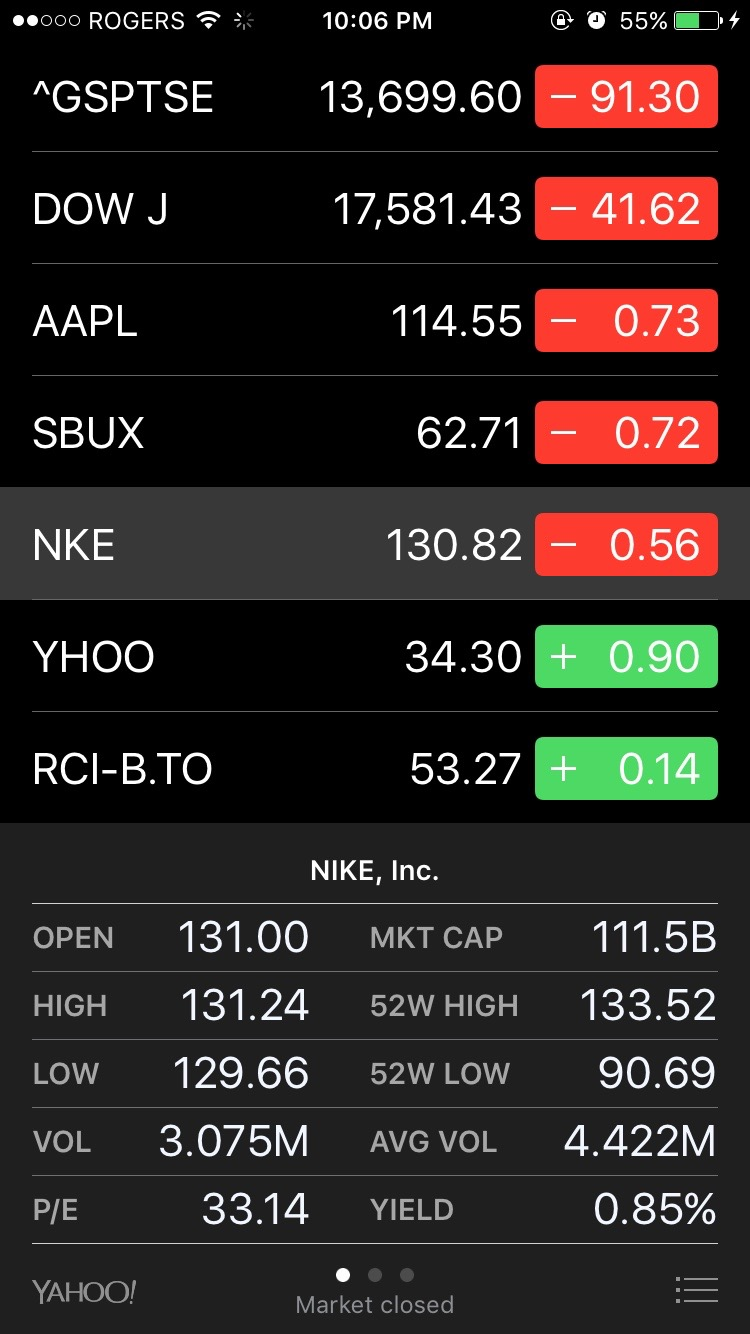
\includegraphics[width=2cm]{today_applestocks.jpg}
%	\caption{The home screen for Apple Stocks. This screen highlights a stock and shows the user the daily values for it.}
%	\label{fig:figure3}
%\end{figure*}
%
%\begin{figure*}
%	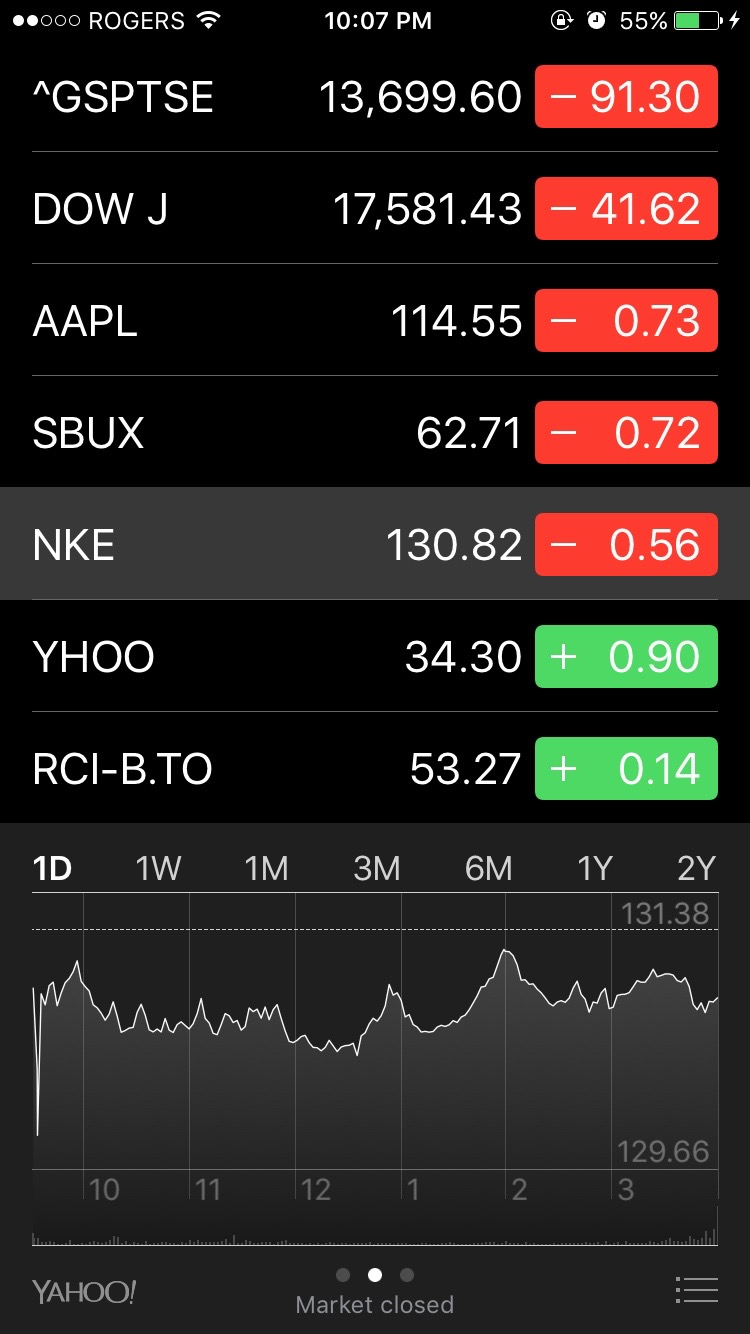
\includegraphics[width=2cm]{dailytrends_applestocks.jpg}
%	\caption{This screen is after the user swipes in the information center for the stock. Currently, the time span for the trend is one day (1D).}
%	\label{fig:figure4}
%\end{figure*}
% 
%\begin{figure*}
%	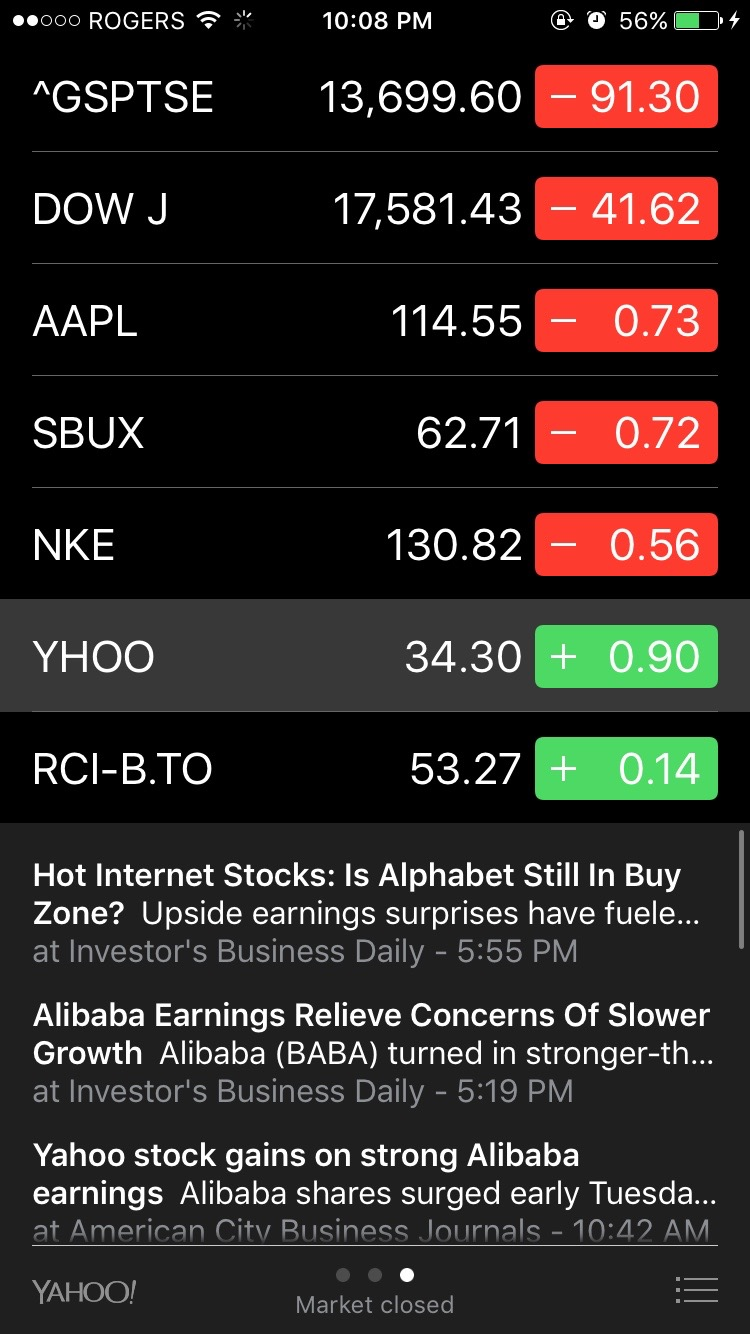
\includegraphics[width=2cm]{relatednews_applestocks.jpg}
%	\caption{This screen is after the user changes the time span for their trend analysis - in this case, it is a six month span (6M). The user can switch between time spans by clicking on the options above the chart.}
%	\label{fig:figure5}
%\end{figure*}
% 
%\begin{figure*}
%	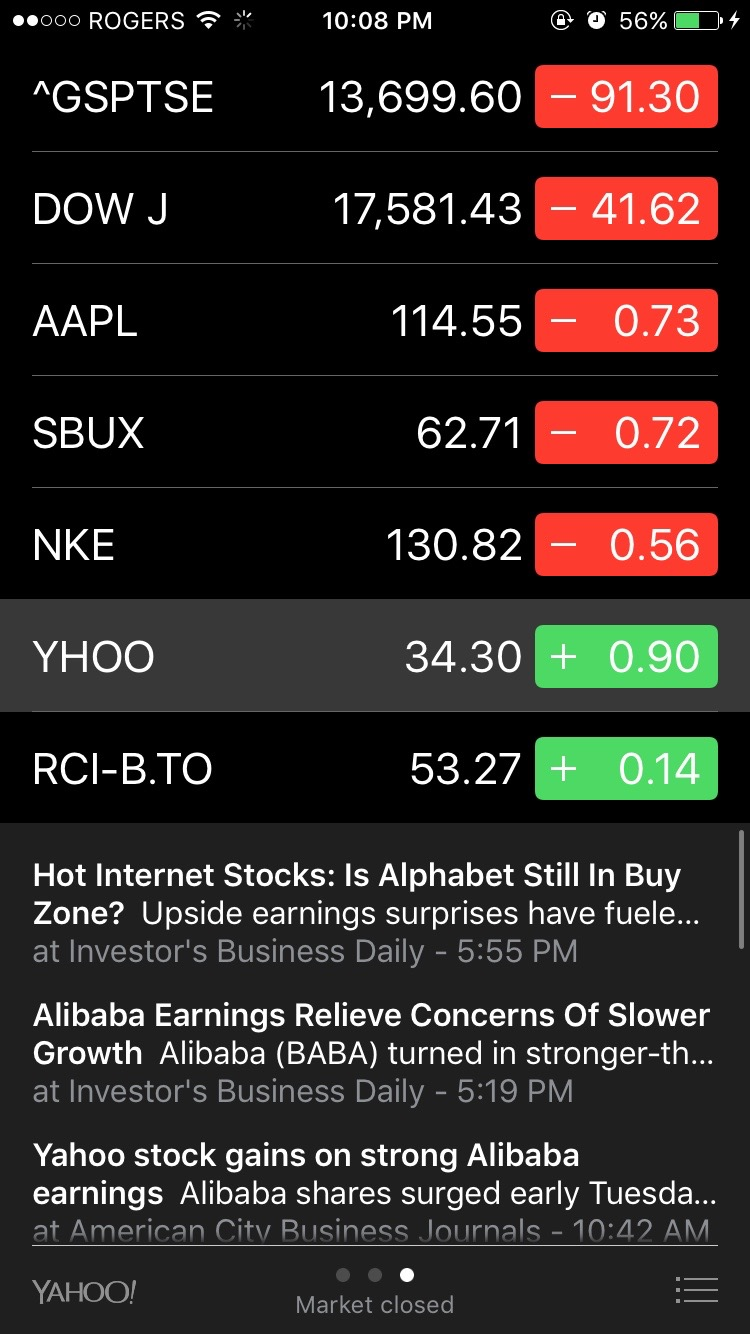
\includegraphics[width=2cm]{relatednews_applestocks.jpg}
%	\caption{The related news section of the information center can be accessed by swiping on the trend chart. This section brings up articles that are relevant to the highlighted stock.}
%	\label{fig:figure6}
%\end{figure*}

\section{Conclusion}
Although all of the surveyed applications share some positive attributes, most of them suffer from common elements. This paper has elaborated on the current user interface issues at hand and proposes changes that could greatly improve the overall user experience. These changes will be implemented and evaluated in the upcoming paper. 

% Balancing columns in a ref list is a bit of a pain because you
% either use a hack like flushend or balance, or manually insert
% a column break.  http://www.tex.ac.uk/cgi-bin/texfaq2html?label=balance
% multicols doesn't work because we're already in two-column mode,
% and flushend isn't awesome, so I choose balance.  See this
% for more info: http://cs.brown.edu/system/software/latex/doc/balance.pdf
%
% Note that in a perfect world balance wants to be in the first
% column of the last page.
%
% If balance doesn't work for you, you can remove that and
% hard-code a column break into the bbl file right before you
% submit:
%
% http://stackoverflow.com/questions/2149854/how-to-manually-equalize-columns-
% in-an-ieee-paper-if-using-bibtex
%
% Or, just remove \balance and give up on balancing the last page.
%
\balance
% REFERENCES FORMAT
% References must be the same font size as other body text.

%\bibliographystyle{acm-sigchi}
%\bibliography{sample}
\end{document}
